% !TeX program = pdflatex
% !TeX encoding = UTF-8
\documentclass[fontsize=11pt, parskip=half]{scrartcl}

%preamble loading packages and so on

%packages
\usepackage{scrlayer-scrpage}
\usepackage[datesep={.}, style=ddmmyyyy]{datetime2}
\usepackage{graphicx}
\usepackage{multicol}
\usepackage[colorlinks=true, urlcolor=blue, linkcolor=black]{hyperref}
\usepackage{amsmath}
\usepackage{mathtools}
\usepackage{listings}
\usepackage{csquotes}
\usepackage{wrapfig}
\usepackage{caption}
\usepackage[a4paper, top=2cm, bottom=2cm, left=2cm, right=2cm]{geometry}
\MakeOuterQuote{"}
\usepackage{array}   % for \newcolumntype macro
\usepackage{multirow}
\newcolumntype{L}{>{$}l<{$}} % math-mode version of "l" column type
\newcolumntype{C}{>{$}c<{$}} % math-mode version of "c" column type
\newcolumntype{R}{>{$}r<{$}} % math-mode version of "r" column type

%%%%%%%%%%%%%%
%commands
%%%%%%%%%%%%%%

%formatting
\renewcommand{\thesubsection}{\thesection.H\arabic{subsection}} %changes subsection labelling to alphabetical -> 1.a instead of 1.1
\captionsetup{labelfont=bf, textfont=it, justification=raggedright,singlelinecheck=false, justification=centering}
%generalmath
\newcommand\br[1]{\ensuremath{\left(#1\right)}}
\newcommand\modulo[1]{\ensuremath{\bmod{\left(#1\right)}}} %adds \modulo{} as command for modulo calculations. Content is placed in brackets.
\DeclarePairedDelimiter\ceil{\lceil}{\rceil} %defines \ceil{} as command producing mathematical ceiling symbols around content
\DeclarePairedDelimiter\floor{\lfloor}{\rfloor} %defines \floor{} as command producing mathematical floor symbols around content
\newcommand\bsum[3]{\ensuremath{\sum_{#1}^{#2}{\left({#3}\right)}}} %defines \bsum{}{}{} as command for large sum with start, end and content. Content is placed in brackets.
\newcommand\bprod[3]{\ensuremath{\prod_{#1}^{#2}{\left({#3}\right)}}} %defines \bprod{}{}{} as command for large product with start, end and content. Content is placed in brackets.
\newcommand\texeq[1]{\stackrel{\mathclap{\normalfont\mbox{\scriptsize {#1}}}}{=}} %defines \teq as command for equal sign with subscript
\newcommand\defeq{\ensuremath{=_{def}}} %defines \defeq as command for definition with equal sign

%formal logic
\newcommand\bland[3]{\ensuremath{\bigwedge_{#1}^{#2}{\left({#3}\right)}}} %defines \bland{}{}{} as command for large logical AND with start, end and content. Content is placed in brackets.
\newcommand\blor[3]{\ensuremath{\bigvee_{#1}^{#2}{\left({#3}\right)}}} %defines \bland{}{}{} as command for large logical OR with start, end and content. Content is placed in brackets.
\newcommand\bforall[2]{\ensuremath{\left(\forall {#1}\right) \left[{#2}\right]}} %defines \bforall{}{} as command for logical forall with variable and content. forall and variable are placed within (), Content is placed in [].
\newcommand\bexists[2]{\ensuremath{\left(\exists {#1}\right) \left[{#2}\right]}} %defines \bexists{}{} as command for logical exists with variable and content. forall and variable are placed within (), Content is placed in [].

%Mathmatical Sets (Mengenlehre)
\newcommand\intenset[2]{\ensuremath{\left\lbrace {#1} \mid {#2} \right\rbrace}} %defines \intenset{}{} as command for intensional notation of mathmatical sets: {@|@}.
\newcommand\intensetU[2]{\ensuremath{\left\lbrace {#1} \in U \mid {#2} \right\rbrace}} %defines \intensetU{}{} as command for intensional notation of mathmatical sets: {@ \in U |@}.
\newcommand\extenset[1]{\ensuremath{\left\lbrace {#1} \right\rbrace}} %defines \extenset{} as command for extensional notation of mathmatical sets: {@}.

% referencing
\newcommand\fref[1]{\textbf{Figure \ref{#1}}} % defines \fref{} as command printing "Figure figurenumber" in bold.

%Title, Author, ...
\makeatletter
\title{Conspiracy narratives and public perception of 15-minute cities on YouTube}\let\Title\@title
\def \papersubtitle {Project Report}
\def \paperdeadline {\href{https://github.com/julia-king-edu/so-24_smda_project}{Link to github repository}}
% seminar information
\def \paperevaluator {Max Pellert}
\def \paperseminar {Social Media Data Analysis}
\def \papersemester {Summer/Winter Semester 2024}
\def \paperdepartment {Department of Politics and Public Administration}
\def \paperuniversity {University of Konstanz}
% personal information
\def \paperemail {julia.king@uni-konstanz.de}
\def \paperprogramme {M.Sc. Social and Economic Data Science}
\def \papermatriculationnr {01/911139}
\author{Julia King}          \let\Author\@author
\date{\today}           \let\Date\@date
\makeatother

% Page Layout
\ihead{Julia K.}
\chead{Conspiracy narratives \& public perception of 15-minute cities on YouTube}
\ohead{SMDA}

% citation setup
\usepackage[style=apa, sorting=nyt, backend=biber]{biblatex}
\usepackage{etoolbox} % If not already included
\addbibresource{citations.bib} %bibliography file


% Custom bibliography driver for article to include howpublished
\DeclareBibliographyDriver{misc}{%
  \printnames{author}%
  \newunit\newblock
  \printfield{year}%
  \newunit\newblock
  \mkbibemph{\printfield{title}}.%
  \newunit\newblock
  \iffieldundef{howpublished}
    {}
    { \href{\thefield{howpublished}}{\thefield{howpublished}}}%
  \newunit\newblock
  \printfield{url}%
}

\begin{document}
\setlength{\columnsep}{25pt}

% Title Page, do not change here, variables are defined above!
\begin{titlepage}
    \newcommand{\HRule}{\rule{\linewidth}{0.5mm}}
    
    \begin{flushleft} % Upper left corner
        \large
        \paperuniversity\\
        \paperdepartment\\
        \papersemester\\
        \paperseminar\\
        \paperevaluator
    \end{flushleft}
    
    \vfill
    
    \begin{center} % Centered title and date
        \huge\bfseries \Title\\
        \vspace{0.5cm}
        \large \papersubtitle \\
        \vspace{0.5cm}
        \small \paperdeadline
    \end{center}
    
    \vfill
    
    \begin{flushright} % Lower right corner
        \large
        \Author\\
        \papermatriculationnr\\
        \paperprogramme\\
        \paperemail
    \end{flushright}
\end{titlepage}

\clearpage
\setcounter{page}{1}

% Main Document
\section{Motivation}
\label{section:motivation}

    The concept of a 15-minute-city is, in and of itself, nothing more than an architectural proposal for efficient and sustainable urban design. However, it rose to prominence during the past five years due to a staggering amount of online conspiracy theories and misinformation. While conspiracy theories often revolve around large events or hard-to-explain phenomena, like the moon landing or many celebrity or politician assassinations, 15-minute-cities are neither. 15-minute-cities, in contrast, are a suggestion in the research field of architecture and city planning, proposing to build new urban developments in a way that ensures residents can reach basic amenities within a 15-minute walking distance. The fact that a simple, academic proposal for city design was (and is) the center of large swathes of online conspiracy theories, is puzzling, and warrants investigation. 
    
    Understanding the puzzling emergence of 15-minute-city conspiracies requires investigation of the ways in which people discussed them publicly. This project aims, therefore, to track the development of theories revolving around this concept by analyzing the online discourse around it. This requires an in-depth understanding of the process in which conspiracy theories took over the discourse on 15-minute-cities. Consequently, this project collects metrics on the viewership of online videos revolving around 15-minute-cities, and to classify the discursive tone of both the videos themselves and the comments posted on them. Using this data, the following hypotheses are tested: 

    \begin{enumerate}
        \item Videos produced before the first spike in public interest are more likely to be non-conspirative compared to those uploaded during and after the spike. \label{h:1}
        \item Comments under conspirative videos express higher levels of negative sentiment compared to comments under non-conspirative videos. \label{h:2}
        \item The engagement metrics (e.g., likes, comments, shares per view) of conspirative videos differ significantly from those of non-conspirative videos, with conspirative videos having higher engagement rates per view. \label{h:3}
    \end{enumerate}

In order to test these hypotheses, this report will first explain the interfaces and resources used to collect the necessary data, before highlighting the data processing steps taken. Afterwards, it will outline and visualize the results of the statistical analyses performed in the project and discuss their validity and reliability. Finally, the report will identify key limitations and alternative explanations for the results.

The code and data used in the project as well as additional visualizations can be found in the \href{https://github.com/julia-king-edu/so-24_smda_project}{github repository}.
    
\section{Data Retrieval}
\label{section:retrieval}

    The following section will outline the various apis and data sources utilized in the project. Specifically, this project gathers data obtained from google trends (\citeyear{google15minuteCity2024}), which is then used to parametrize queries for the Youtube Data api (\citeyear{googlefordevelopersYoutubeDataApi2024}). Finally, the huggingface api (\citeyear{huggingfaceTransformers2024}) is utilized to allow sentiment classification via LEIA.

    In order to track the development of the conspiracy theory and test hypotheses \ref{h:1} and \ref{h:2}, an investigation of the progression of public attention was necessary. In line with previous research (including \cite{mavraganiAssessingMethodsTools2018,yeoPublicAttentionLocal2019,junTenYearsResearch2018a}), Google Trends data was chosen to model public interest and identify relevant phases of the conspiracy. Obtained via the pytrends package \parencite{dreyco676Pytrends2023} in python \parencite{vanrossumPythonReferenceManual2009}, the data was limited to the United States of America, as the conspiracy itself was highly focussed on the country. Additionally, Google Trends distinguishes between search terms and topics, with topics also including variants of the given term. Thus, the query was specified for the 15-minute city topic.

    \begin{figure}{}
        \centering
        \setlength\intextsep{0pt}
        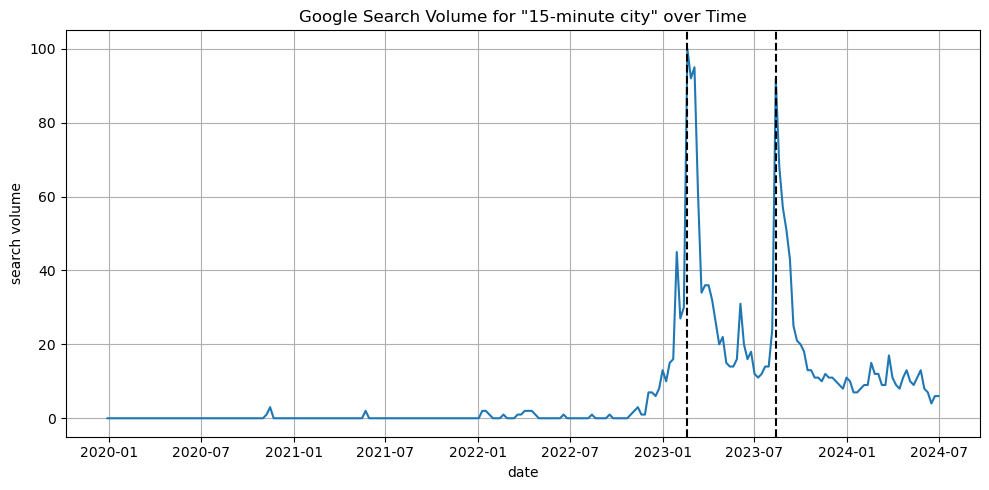
\includegraphics[width=0.8\textwidth]{img/gtrends_2-peak.png}
        \vspace{-5pt}
        \caption{Public interest in 15-minute cities measured by search volume}
        \vspace{-10pt}
        \label{fig:gtrends_raw}
    \end{figure}

    The results of the Google Trends data collection, visualized in figure \ref{fig:gtrends_raw}, were crucial to the parametrization of the youtube api requests. Specifically, distinct phases centered around the presence or absence of a peak in public interest were algorithmically identified to ensure all relevant data was obtained while preventing excessive use of the api. For now, it is important to note that this procedure, the details of which will be discussed in \nameref{section:processing}, also yielded a cutoff-point before the first relevant phase.

    Following the google trends data collection, multiple endpoints of the YouTube Data Api were utilized to obtain relevant data on the most-viewed videos regarding 15-minute cities. First, the \textit{search} endpoint was employed to identify the 50 most-viewed videos per week. This weekly structure, while quota-intensive, enabled the identification of temporal trends in the analysis stage and was thus crucial for this project. Afterwards, metadata on all of the identified videos was obtained using the \textit{video} endpoint. Finally, multiple queries to the \textit{commentThread} endpoint per video allowed for the collection of all top-level comments under all videos. The data collection and analysis was limited to top-level comments, as those should provide the most accurate reflection of the audience reactions to the given video, instead of reactions to other comments.
    
    In total, 119 weeks of videos were processed, resulting in a dataset containing information on 2943 videos and 204093 comments, a process that required multiple days due to the quota limits imposed by the YouTube Data API. Note that some weeks, especially those before the first spike in public attention, did not have 50 new videos uploaded, leading to a smaller number of videos collected for those weeks. Despite this, the dataset still provides more than adequate data for analyzing the progression of the conspiracy theory surrounding 15-minute cities. 

    Finally, the huggingface api was utilized to obtain the LEIA-base transformer model \parencite{aroyehunLEIALinguisticEmbeddings2023}, which was later employed to classify the sentiments of the comments obtained via the YouTube Api. In addition to its performance in the assignments completed for this course, the LEIA-base model was chosen due to its ability to classify natural language sentiment in a fine-grained manner, distinguishing between Affection, Happiness, Anger, Sadness and Fear instead of a simple polarity score. This distinction of LEIA when compared to other sentiment analysis techniques such as VADER \parencite{cjhuttoVaderSentiment2020} is especially relevant in the context of conspiracy theories, as a comment expressing sadness implies a much lower threat level than a comment expressing anger. Thus, utilizing LEIA-base enables the generation of additional inferences into the conspiracy by providing a more fine-grained perspective.

\section{Data Processing}
\label{section:processing}

    The Google Trends data  was utilized to identify distinct phases in public interest, enabling the progression of key variables during different stages of development of the conspiracy theory. Differences in rolling averages were used to identify the beginning and end of peaks, with steady increases indicating the beginning of a spike and the end of a steady decrease defining the end of a spike. As seen in figure \ref{fig:gtrends_phases}, four distinct phases were identified: 
    \begin{enumerate}
        \item The phase before the first spike, which is hypothesized to contain mostly educational videos on the concept of 15-minute cities.
        \item The first spike, hypothesized to be caused by the rise of conspirative content.
        \item The second spike, hypothesized to be caused by mainstream media coverage.
        \item The phase after both spikes, where search volume has returned to a steady level.
    \end{enumerate}

    \begin{figure}{}
        \centering
        \setlength\intextsep{0pt}
        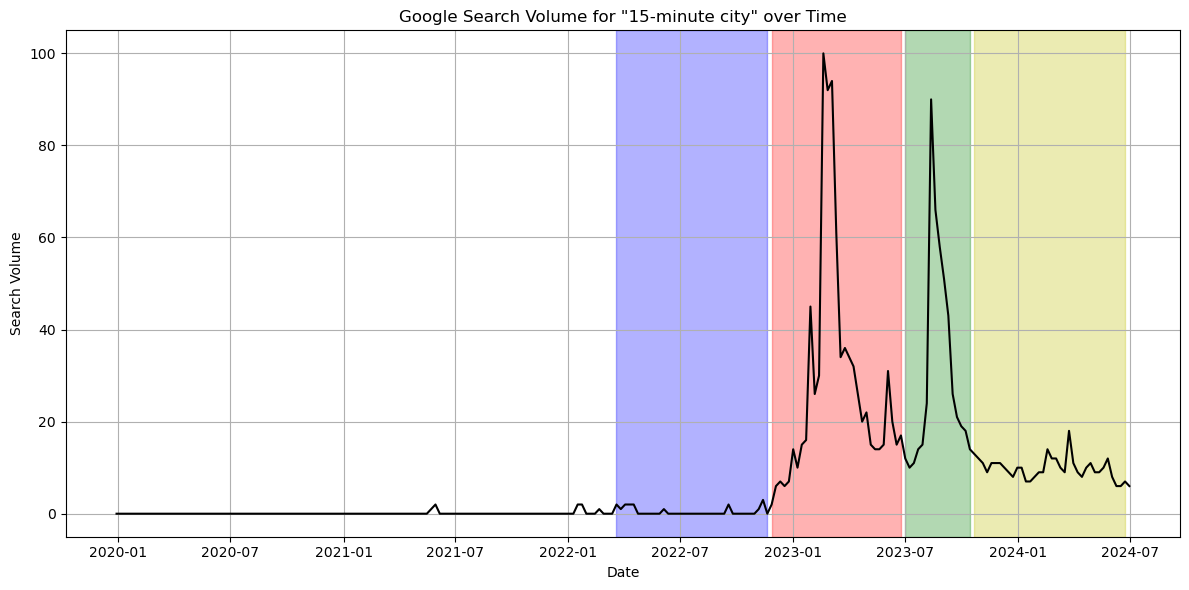
\includegraphics[width=0.8 \textwidth]{img/gtrends_phases.png}
        \vspace{-5pt}
        \caption{Visualization of the generated phases}
        \vspace{-10pt}
        \label{fig:gtrends_phases}
    \end{figure}

    Following the identification of phases, a random sample from the results of the \textit{videos} endpoint was drawn and designated for manual classification into conspirative and non-conspirative content. This classification was conducted using a tkinter app, which presented the rater with the title and description of a given video. A link to the full video was also provided for cases where unambiguous classification based on the previous attributed was not possible. In total, 400 videos were classified, allowing for a train-test split of 300/100 videos.

    In order to facilitate automatic classification via supervised learning techniques, the video's titles and descriptions were preprocessed. This included the removal of links, newlines, non-alphanumeric characters and stopwords, as well as tokenizing and lemmatizing. These cleaned versions were included in a dataframe containing video-level information. This dataframe also included the phase, week of upload, video id, raw versions of the video's title and description as well as the number of views, likes and comments. Sadly, the number of times a video has been shared is no longer reported in the video metadata. Thus, hypothesis \ref{h:3} can only be tested with regards to likes and comments per view.

    In order to ensure the best possible performance, multiple supervised learning techniques were applied and evaluated. Specifically, the approaches employed by this project include the (Gaussian) Naive Bayes, Support Vector Machine and Random Forest algorithms from the sklearn python package \parencite{pedregosaScikitlearnMachineLearning2011}. All three models were fitted using the 300 tweets in the training data and evaluated based on their performance on the test set. The evaluations informed the final model choice and are not part of the substantial analysis and are thus presented in this section. 

    \begin{wrapfigure}{r}{0.5\textwidth}
        \setlength\intextsep{0pt}
        \vspace{-10pt}
        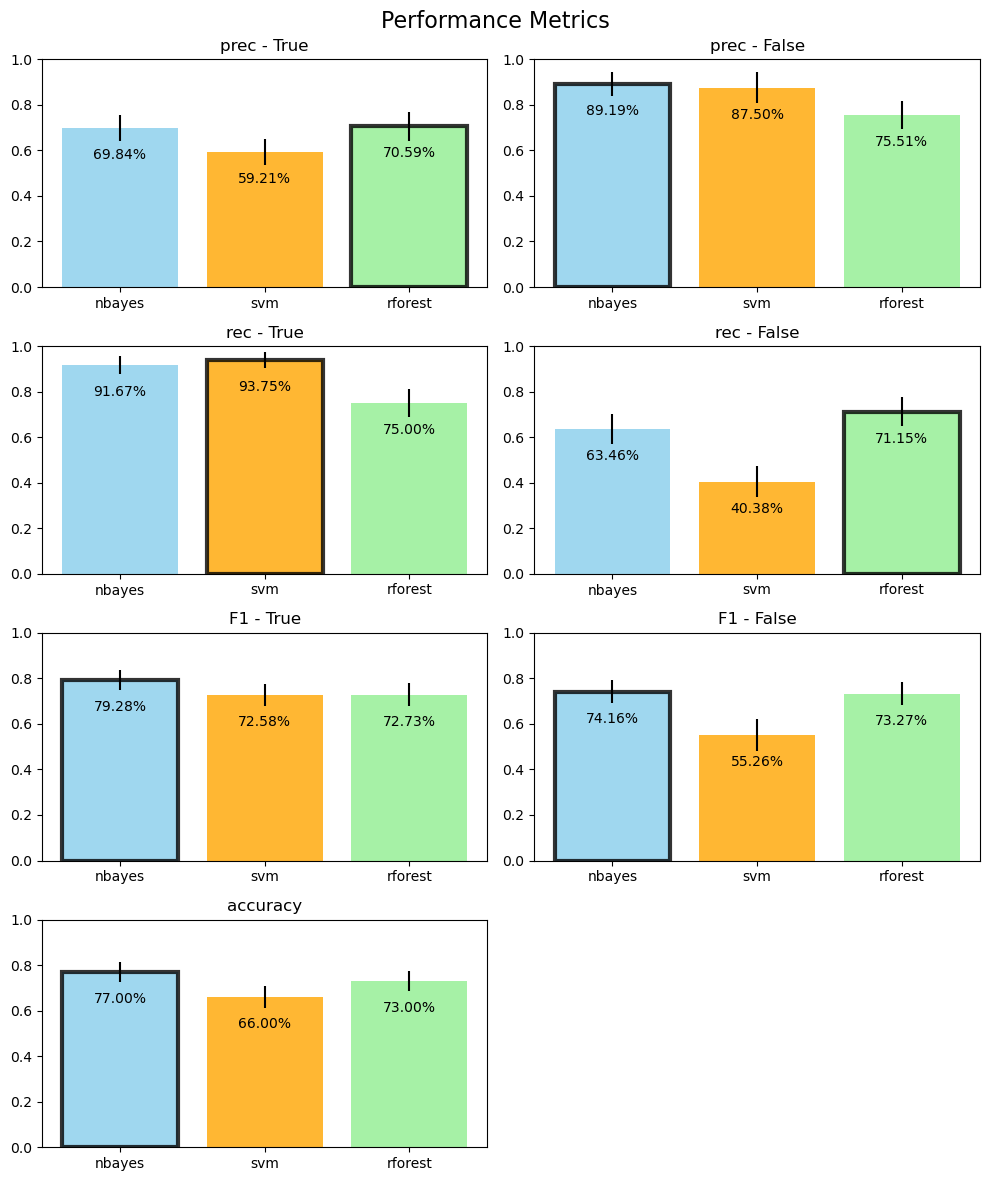
\includegraphics[width=0.48 \textwidth]{img/labels_performance.png}
        \vspace{-5pt}
        \caption{Performance metrics of supervised learning models}
        \vspace{-10pt}
        \label{fig:performance}
    \end{wrapfigure}

    Based on the performance metrics visualized in \ref{fig:performance}, the Naive Bayes classifier was selected, as it provided the highest accuracy as well as the highest F1-scores in the sample. However, based on the uncertainty estimates plotted above, it is important to highlight that this performance was no statistically significant advantage of Naive Bayes when compared to other algorithms, with especially the random forest algorithm often performing similarly. Thus, other training and testing samples may have resulted in the selection of a different model. The model was then used to automatically classify all 2943 videos, with the classifications being added to the video dataframe. 

    Finally, the emotion classification model LEIA was applied to obtain the sentiments expressed in each of the 204093 top-level comments. This also involved the creation of a new dataframe saving comment-level information including the phase, week and video id of the comment, as well as the comment id and text. Notably, the comment texts were not cleaned before classification as to preserve important contextual information, which can be utilized by LEIA (in contrast to the supervised learning models above). The classification was done on a local machine over several hours.
    
\section{Analysis}
\label{section:analysis}

    The following analysis section will group the findings of the project by hypothesis.

    \subsection{Videos produced before the first spike in public interest are more likely to be non-conspirative compared to those uploaded during and after the spike.}

    \begin{wrapfigure}{r}{0.6\textwidth}
        \centering
        \vspace{-20pt}
        \setlength\intextsep{0pt}
        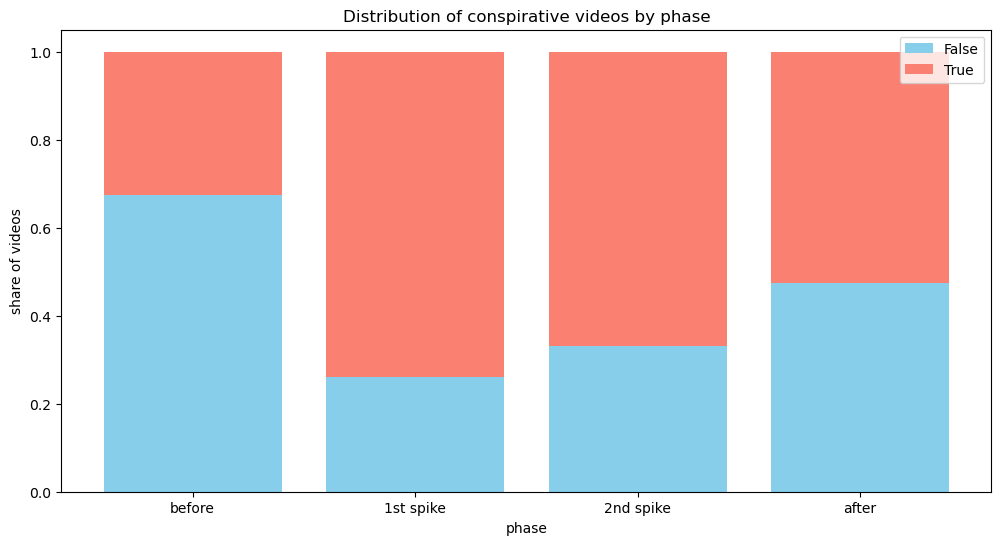
\includegraphics[width=0.58 \textwidth]{img/conspirative_phase.png}
        \vspace{-5pt}
        \caption{Share of conspiracy narratives per phase}
        \vspace{-10pt}
        \label{fig:conspiracy_phase}
    \end{wrapfigure}

    To test this hypothesis, a contingency table of the variables \textit{video phase} and \textit{conspirative} was constructed. A normalized version of this table is visualized in \ref{fig:conspiracy_phase}. In line with the hypothesis, the phase before the first spike in public expressed the lowest share of conspirative content. Notably, the share of conspirative content staded above 50\% for all following phases. This runs counter to the theory outlined in the \nameref{section:processing} section, as an influx in mass media attention should've also increased the amount of informative content debunking the conspiracy theory. Nevertheless, the tendencies predicted by the hypothesis are found in the data.
    
    After this exploratory analysis, a test for statistical independence of two categorical variables was conducted. Due to the large sample size and differing group sizes, Pearson's Chi-squared test was chosen. Two variants of the test were conducted: Test 1a was based on a dataset distinguishing between all 4 phases, while test 1b was conducted by first grouping the data of phases 2, 3 and 4 together to more closely align with the hypothesis above. Both tests were highly significant, with Chi-square statistics of $210.93$ ($p < 0.001$) and $108.13$ ($p < 0.001$) respectively. Thus, this project was able to confidently reject the null hypothesis, showcasing a significant increase in conspirative content.    

    In addition to the per-phase analysis conducted in the above test, a continuous visualization of the progression of the rate of conspirative content was generated. The findings are presented in the additional figures provided in the \href{https://github.com/julia-king-edu/so-24_smda_project}{github repository}. 

    \subsection{Comments under conspirative videos express higher levels of negative sentiment compared to comments under non-conspirative videos.}

    \begin{wrapfigure}{r}{0.6\textwidth}
        \centering
        \vspace{-20pt}
        \setlength\intextsep{0pt}
        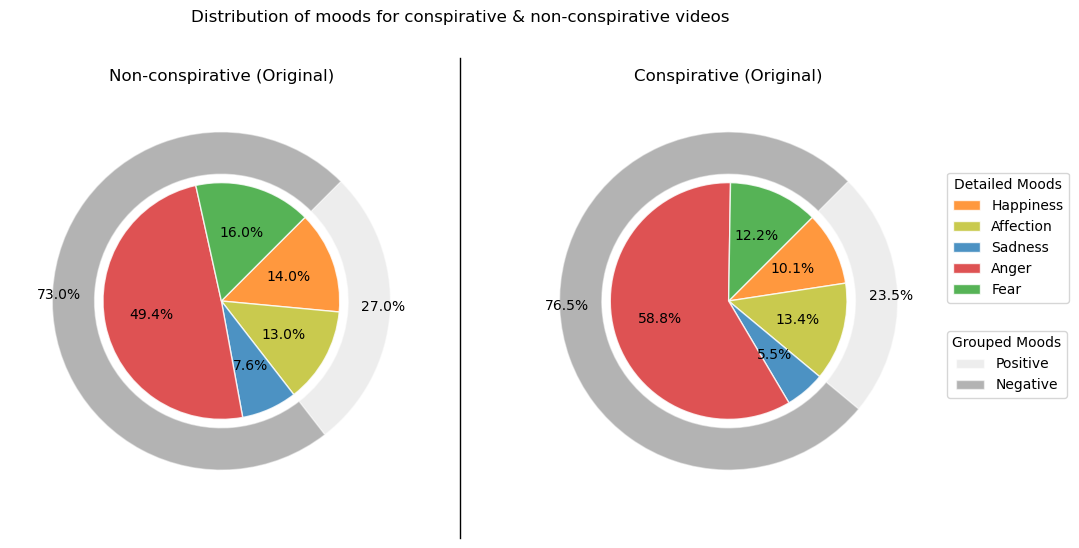
\includegraphics[width=0.58 \textwidth]{img/moods_conspirative-pie.png}
        \vspace{-5pt}
        \caption{Distribution of comment moods by conspirative classification}
        \vspace{-10pt}
        \label{fig:moods_conspirative-pie}
    \end{wrapfigure}

    To explore this hypothesized connection, the distribution of sentiments in the comments of conspirative and non-conspirative videos was visualized in figure \ref{fig:moods_conspirative-pie}. Significant differences in the distribution of detailed moods are observable. This is especially pronounced when observing the sentiment anger, which increases from 49\% for non-conspirative videos to 59\% for conspirative videos. However, the differences in grouped moods are much less pronounced, only differing by about 3\%. While the direction of this change is consistent with the hypothesis outlined above, the small magnitude of this difference is noteworthy.

    Nevertheless, two Chi-squared test were conducted, one for the detailed sentiments and one with a polarity grouping matching the hypothesis above, were conducted. Once again, both tests revealed highly significant correlations, with Chi-square statistics of $1761.02$ ($p < 0.001$) and $242.75$ ($p < 0.001$) respectively. These results can be explained by the large sample size (204093 comments in total), as large samples are able to establish significance even if the differences in group means are minimal.

    \subsection{The engagement metrics (e.g., likes, comments, shares per view) of conspirative videos differ significantly from those of non-conspirative videos, with conspirative videos having higher engagement rates per view.}

    \begin{wraptable}{r}{0.3\textwidth}
        \begin{tabular}{ll|ll|}
        \cline{3-4}
                                                                                                          &          & \multicolumn{2}{l|}{conspirative} \\ \cline{3-4} 
                                                                                                          &          & True            & False           \\ \hline
        \multicolumn{1}{|l|}{\multirow{2}{*}{\begin{tabular}[c]{@{}l@{}}metric \\ per view\end{tabular}}} & likes    & 0.052           & 0.026           \\
        \multicolumn{1}{|l|}{}                                                                            & comments & 0.004           & 0               \\ \hline
        \end{tabular}
        \caption{Median engagement metrics}
        \label{table:median_metrics}
    \end{wraptable}

    In order to test this hypothesis, per-view metrics were created and tested for normality. Notably, this required the exclusion of 122 videos, which featured obviously erroneous query results, including more like and/or comments than views. Visual inspection of the figures plotting the distributions of likes and comments per view (which can be found in the \href{https://github.com/julia-king-edu/so-24_smda_project}{github repository}) revealed strong non-normal distributions, even when logged. Thus, table \ref{table:median_metrics} shows the median engagement metrics per view. In line with our hypothesis, they are higher for conspirative videos.
    
    Due to the aforementioned non-normalcy of the distributions, a nonparametric test was chosen instead of a traditional t-test. Specifically, the Mann-Whitney U rank test was employed, as it compares rank sums instead of means, allowing for non-normal distributions to be compared. Both tests yielded highly significant results, with U-statistics of $1169852.5$ ($p < 0.001$) for likes and $1064695.5$ ($p < 0.001$) for comments. Therefore, we find significant evidence of increased engagement with conspirative videos.    

\section{Conclusion}
\label{section:conclusion}

    This project found statistically significant evidence for all three main hypohteses outlined in the research proposal. First, it established that conspirative content rapidly increased during the first spike in public attention. This sudden influx may indicate an audience overlap with preceeding conspiracy theories, as the 15-minute city conspiracy theory may have been shared in those channels. Further evidence for this can be found in the fact that conspirative videos in the dataset often refer to other conspiracy theories, including the New World Order conspiracy theory (see \cite{sparkConjuringOrderNew2000}). 

    Second, the project finds evidence of increased negative sentiment in the comments of conspirative videos. However, as outlined in the previous section, the substantive difference between the two groups was minimal when only observing sentiment valence, and significantly increased when introducing additional emotion dimensions. Thus, the reliability and generalizability of hypothesis \ref{h:2} is severely diminished by the oversimplification of the emotion space when observing reactions to conspiracy theories and future project should utilize a more detailed operationalization.

    Third, conspirative videos in the sample experienced significantly higher levels of engagement per view. This discovery is in line with previous research, which has shown other kinds of engagement inspired by conspiracy theories, including political engagement \parencite{kimHowConspiracyTheories2022}. However, the findings here only pertain to the most-viewed videos per week and can thus not be generalized to all conspirative videos. 

\section{Critique}
\label{section:critique}

    \textcolor{red}{Identify limitations and alternative explanations for your results.}

    As mentioned in the \nameref{section:analysis} section, the calculation of per-view metrics revealed undeniably erroneous data provided by the YouTube Data api, including instances where likes exceed view counts by factors of up to 5. Notably, these errors are also present on the YouTube website (\href{https://www.youtube.com/watch?v=XVKdKDHH7UE}{see this video for an example}) and thus not caused by errors in the project. Nevertheless, these discrepancies might impact the results, especially if such errors also occur in the non-detectable range, for instance with inflated like counts that do not exceed the view count.

    Additionally, while the increase in google searches coincides with an increased share of conspirative YouTube videos, the causality of these events is unclear. Thus, it is possible that the sharp increase in conspirative content was not the product of organically occuring public attention but instead of thought leaders engaged in the wider "conspiracy bubble" promoting the 15-minute city conspiracy theory. Consequently, a qualitative analysis of early conspirative videos may reveal further insights into the emergence of conspiracy theories not pertaining to large events or hard-to-explain phenomena.

    Finally, this project conducted extensive testing of the applied supervised learning techniques to ensure the usage of a well-performing model. However, the performance metrics (see figure \ref{fig:performance}) reveal imbalances between the labels for all three algorithms, with significantly higher recall and lower precision for conspirative videos, which may have lead to an overestimation of conspirative content and could inflate the results. Future projects should thus expand on model selection to aim for a closer match to the data.    

\newpage

\onecolumn
\begin{minipage}[t]{\textwidth}
    \printbibliography[heading=bibintoc, title={References}]
\end{minipage}


\end{document}
